\documentclass[aspectratio=169]{beamer}

% Shared Beamer settings for Elements of AIML lectures (UPES).
% Keep this file free of \documentclass to allow reuse via \input.

% Allow lecture sources to use shared theme/assets without copying them into each lecture folder.
% NOTE: These paths are relative to `Unit-xx/Lecture-yy/latex/` (and `Lab/Experiment-xx/latex/`).
\makeatletter
\def\input@path{{../../../_shared/}{../../../_shared/UPES-Beamer-Theme/}}
\makeatother

\usetheme{UPES}
\setbeamertemplate{navigation symbols}{}

\usepackage{amsmath}
\usepackage{amssymb}
\usepackage{booktabs}
\usepackage{graphicx}
\usepackage{hyperref}
\usepackage{xcolor}
\usepackage{listings}

% Code listings (general-purpose).
\lstset{
  basicstyle=\ttfamily\small,
  keywordstyle=\color{blue},
  commentstyle=\color{gray},
  stringstyle=\color{teal},
  showstringspaces=false,
  columns=fullflexible,
  breaklines=true
}

\usepackage{tikz}
\usetikzlibrary{arrows.meta,positioning,shapes.geometric,calc}

% Per-slide source line (references shown on the slide itself).
\newcommand{\slidesources}[1]{%
  \vfill
  {\tiny\color{gray}\raggedright\sloppy\parbox{\linewidth}{Sources: #1}\par}%
}

% Unit-wise source strings for this subject (used by slides/notes).
% Path is relative to the lecture `latex/` folder (the compilation CWD).
% Source strings for Elements of AIML (used by slides + notes).

\newcommand{\AIMLRepoURL}{https://github.com/tali7c/Elements-of-AIML}

\newcommand{\AIMLLabSources}{%
Provost and Fawcett, \textit{Data Science for Business}.;%
McKinney, \textit{Python for Data Analysis}.;%
WEKA Documentation (Waikato Environment for Knowledge Analysis), accessed 2026-02-28.;%
Matplotlib and Seaborn documentation, accessed 2026-02-28.%
}

\newcommand{\AIMLUnitISources}{%
Rich and Knight, \textit{Artificial Intelligence}, McGraw Hill, 2017.;%
Russell and Norvig, \textit{Artificial Intelligence: A Modern Approach} (4e), Ch. 1--2 (Introduction, Intelligent Agents).;%
Poole and Mackworth, \textit{Artificial Intelligence: Foundations of Computational Agents} (2e), selected sections.%
}

\newcommand{\AIMLUnitIISources}{%
Russell and Norvig, \textit{Artificial Intelligence: A Modern Approach} (4e), Ch. 7--9 (Logical Agents, First-Order Logic, Inference).;%
Huth and Ryan, \textit{Logic in Computer Science} (2e), selected sections on propositional and first-order logic.;%
Genesereth and Nilsson, \textit{Logical Foundations of Artificial Intelligence}, selected chapters.%
}

\newcommand{\AIMLUnitIIISources}{%
Mueller and Massaron, \textit{Machine Learning for Dummies}, For Dummies, 2016.;%
Mitchell, \textit{Machine Learning}, selected chapters on learning basics and evaluation.;%
Scikit-learn documentation, accessed 2026-02-28.%
}

\newcommand{\AIMLUnitIVSources}{%
Mueller and Massaron, \textit{Machine Learning for Dummies}, For Dummies, 2016.;%
James, Witten, Hastie, and Tibshirani, \textit{An Introduction to Statistical Learning} (2e), selected chapters.;%
Scikit-learn documentation, accessed 2026-02-28.%
}

\newcommand{\AIMLUnitVSources}{%
NIST, \textit{AI Risk Management Framework (AI RMF 1.0)}, 2023.;%
Barocas, Hardt, and Narayanan, \textit{Fairness and Machine Learning} (online book), selected sections.;%
Knaflic, \textit{Storytelling with Data}, selected chapters on communicating results.%
}



\title[Elements of AIML]{Elements of AIML}
\subtitle{Unit 01 -- Lecture 01: AI Overview, Techniques \& Applications}
\author{Tofik Ali}
\institute{School of Computer Science, UPES Dehradun}
\date{\today}

\graphicspath{{../images/}{../../../_shared/}{../../../_shared/UPES-Beamer-Theme/}}

\begin{document}

\UPESCoverFrame
\setcounter{framenumber}{0}

\begin{frame}
  \titlepage
  \vspace{0.3em}
  \begin{center}
    \footnotesize Topic focus: \textbf{What is AI?} where it is used, and how to judge success\\[0.25em]
    \footnotesize Repository: \texttt{\AIMLRepoURL}
  \end{center}
  \slidesources{\AIMLUnitISources}
\end{frame}

\begin{frame}{Quick Links}
  \centering
  \hyperlink{sec:overview}{\beamerbutton{Overview}}\hspace{0.6em}
  \hyperlink{sec:apps}{\beamerbutton{Applications}}\hspace{0.6em}
  \hyperlink{sec:models}{\beamerbutton{Models}}\hspace{0.6em}
  \hyperlink{sec:example}{\beamerbutton{Example}}\hspace{0.6em}
  \hyperlink{sec:summary}{\beamerbutton{Summary}}
\end{frame}

\begin{frame}{Agenda}
  \tableofcontents
\end{frame}

\section{Overview}
\label{sec:overview}

\begin{frame}{Learning Outcomes}
  By the end of this lecture, you should be able to:
  \begin{itemize}[<+->]
    \item Explain what \textbf{Artificial Intelligence (AI)} means using at least two viewpoints.
    \item Differentiate \textbf{AI vs ML vs Data Science} with simple examples.
    \item List common \textbf{AI technique families} (symbolic, statistical, hybrid) and when each is used.
    \item Describe what a \textbf{model} is and outline \textbf{criteria of success} beyond accuracy.
  \end{itemize}
\end{frame}

\begin{frame}{Course Roadmap (Units I--V)}
  \begin{itemize}[<+->]
    \item \textbf{Unit I:} What is AI? techniques, intelligent agents, impact and domains.
    \item \textbf{Unit II:} Logic for AI (propositional logic, predicate logic, entailment, resolution, unification).
    \item \textbf{Unit III:} ML basics (datasets, features, splitting, cross-validation, PCA/LDA/ICA).
    \item \textbf{Unit IV:} ML types (regression, classification, clustering, RL, semi-supervised).
    \item \textbf{Unit V:} Applications + responsible AI considerations.
  \end{itemize}
\end{frame}

\begin{frame}{Abbreviations (Used in This Lecture)}
  \begin{itemize}[<+->]
    \item \textbf{AI}: Artificial Intelligence
    \item \textbf{ML}: Machine Learning
    \item \textbf{DS}: Data Science
    \item \textbf{EDA}: Exploratory Data Analysis (used in labs)
    \item \textbf{KB}: Knowledge Base (used heavily in Unit II)
  \end{itemize}
\end{frame}

\begin{frame}{Why AI ``Works'' Today (Three Drivers)}
  \begin{itemize}[<+->]
    \item \textbf{Data}: large-scale digital data (text, images, transactions, sensors)
    \item \textbf{Compute}: GPUs/TPUs + distributed computing + cheaper storage
    \item \textbf{Algorithms}: better optimization, architectures, and tooling
  \end{itemize}
  \vspace{0.4em}
  Practical takeaway: AI performance depends on \textbf{data + compute + modeling choices}, not only on algorithms.
\end{frame}

\begin{frame}{What is AI? (Four Common Views)}
  \begin{itemize}[<+->]
    \item \textbf{Thinking humanly}: model human cognition (cognitive science view)
    \item \textbf{Acting humanly}: behave like humans (e.g., Turing Test view)
    \item \textbf{Thinking rationally}: reason correctly using logic
    \item \textbf{Acting rationally}: choose actions that maximize goal achievement
  \end{itemize}
  \vspace{0.4em}
  \begin{block}{Working definition (for this course)}
    AI is the study and engineering of \textbf{systems that perceive, reason, learn, and act} to achieve goals in their environment.
  \end{block}
\end{frame}

\begin{frame}{AI vs ML vs Data Science (Quick Contrast)}
  \begin{itemize}[<+->]
    \item \textbf{AI}: broad goal --- build intelligent behavior (reasoning, planning, perception, learning).
    \item \textbf{ML}: subset of AI --- learn patterns from data to make predictions/decisions.
    \item \textbf{Data Science}: extract insights/value from data (analysis, visualization, experimentation).
  \end{itemize}
  \vspace{0.4em}
  \begin{exampleblock}{Example}
    Spam filtering: rule-based filters (AI), learned classifier (ML), reporting spam trends (data science).
  \end{exampleblock}
\end{frame}

\begin{frame}{AI Techniques (High-Level Buckets)}
  \begin{itemize}[<+->]
    \item \textbf{Symbolic AI}: explicit rules/knowledge (logic, search, planning)
    \item \textbf{Statistical AI / ML}: learn from examples (regression, classification, clustering)
    \item \textbf{Hybrid}: combine rules + learning (common in real systems)
  \end{itemize}
  \vspace{0.4em}
  Typical question:
  \[
    \textit{``Do we know the rules? If not, can we learn them from data?''}
  \]
\end{frame}

\begin{frame}{Symbolic vs Statistical vs Hybrid (Comparison)}
  \centering
  \begin{tabular}{p{3.4cm}p{4.3cm}p{4.3cm}}
    \toprule
    \textbf{Approach} & \textbf{Strengths} & \textbf{Limitations} \\
    \midrule
    Symbolic (rules/logic) &
    Interpretable; uses explicit knowledge; strong constraints &
    Hard to scale to messy data; brittle if rules incomplete \\
    \midrule
    Statistical / ML &
    Learns from data; handles noisy patterns; adapts with retraining &
    Needs data; can be biased; harder to explain; sensitive to drift \\
    \midrule
    Hybrid &
    Combines constraints + learning; often best in practice &
    More engineering; needs careful integration and monitoring \\
    \bottomrule
  \end{tabular}
\end{frame}

\begin{frame}{AI Task Types (What the System Outputs)}
  \begin{itemize}[<+->]
    \item \textbf{Classification:} choose a label (spam/not spam)
    \item \textbf{Regression:} predict a number (house price)
    \item \textbf{Ranking / recommendation:} order items (top videos to show)
    \item \textbf{Clustering:} group similar examples (customer segments)
    \item \textbf{Decision making:} choose an action (agent behavior)
  \end{itemize}
  \vspace{0.4em}
  Many ``applications'' are the same core tasks applied to different domains.
\end{frame}

\section{Applications}
\label{sec:apps}

\begin{frame}{Where AI is Used (Examples)}
  \begin{itemize}[<+->]
    \item \textbf{Healthcare}: triage, imaging assistance, risk prediction
    \item \textbf{Finance}: fraud detection, credit scoring, customer support
    \item \textbf{Security}: anomaly detection, spam/phishing detection
    \item \textbf{Education}: personalization, content recommendation
    \item \textbf{Logistics}: demand forecasting, route optimization
  \end{itemize}
  \vspace{0.4em}
  Key idea: most applications reduce to tasks like \textbf{prediction}, \textbf{ranking}, \textbf{classification}, or \textbf{decision making}.
\end{frame}

\begin{frame}{From Domain to ML Task (Example Mapping)}
  \begin{itemize}[<+->]
    \item \textbf{Banking} $\rightarrow$ fraud detection $\rightarrow$ imbalanced classification
    \item \textbf{Healthcare} $\rightarrow$ risk prediction $\rightarrow$ classification/regression + safety constraints
    \item \textbf{Retail} $\rightarrow$ demand forecasting $\rightarrow$ regression + drift (seasonality)
    \item \textbf{Security} $\rightarrow$ intrusion detection $\rightarrow$ anomaly detection + adversaries
  \end{itemize}
\end{frame}

\begin{frame}{Typical AI System Pipeline}
  \centering
  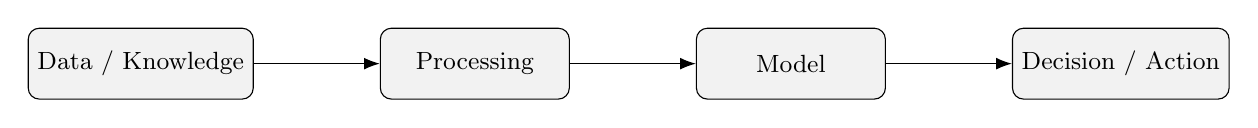
\begin{tikzpicture}[node distance=1.6cm, every node/.style={font=\small}]
    \node (data) [draw, rounded corners, fill=gray!10, minimum width=2.4cm, minimum height=0.9cm] {Data / Knowledge};
    \node (prep) [draw, rounded corners, right=of data, fill=gray!10, minimum width=2.4cm, minimum height=0.9cm] {Processing};
    \node (model) [draw, rounded corners, right=of prep, fill=gray!10, minimum width=2.4cm, minimum height=0.9cm] {Model};
    \node (deploy) [draw, rounded corners, right=of model, fill=gray!10, minimum width=2.4cm, minimum height=0.9cm] {Decision / Action};
    \draw[-{Latex[length=2mm]}] (data) -- (prep);
    \draw[-{Latex[length=2mm]}] (prep) -- (model);
    \draw[-{Latex[length=2mm]}] (model) -- (deploy);
  \end{tikzpicture}
  \vspace{0.4em}
  \begin{itemize}
    \item In Unit II we focus on \textbf{knowledge} + \textbf{logic-based inference}.
    \item In Units III--IV we focus on \textbf{data} + \textbf{learning from examples}.
  \end{itemize}
\end{frame}

\section{Models and Success Criteria}
\label{sec:models}

\begin{frame}{What is a Model? (Levels)}
  A \textbf{model} is a simplified representation of reality used for reasoning or prediction.
  \vspace{0.4em}
  \begin{itemize}[<+->]
    \item \textbf{Conceptual level}: diagrams, assumptions, ``what matters'' (whiteboard model)
    \item \textbf{Mathematical level}: equations/objective functions (e.g., loss)
    \item \textbf{Algorithmic level}: procedures (training, inference, search)
    \item \textbf{System level}: code + data pipeline + monitoring in production
  \end{itemize}
\end{frame}

\begin{frame}{Criteria of Success (Beyond Accuracy)}
  \begin{itemize}[<+->]
    \item \textbf{Correctness/Quality}: accuracy, error rates, calibration
    \item \textbf{Cost}: compute, memory, energy, data collection cost
    \item \textbf{Speed}: latency and throughput
    \item \textbf{Robustness}: stability under noise and changing data
    \item \textbf{Fairness \& Safety}: bias, harmful outcomes, privacy
    \item \textbf{Maintainability}: monitoring, retraining, drift handling
  \end{itemize}
\end{frame}

\begin{frame}{Offline vs Online Success (Reality Check)}
  \begin{itemize}[<+->]
    \item Offline: evaluation on held-out test set (Unit III).
    \item Online: performance in deployment (users, drift, constraints).
    \item A model can have great test accuracy but still fail due to:
      \begin{itemize}
        \item wrong metric for the real cost,
        \item bias/fairness issues,
        \item changing data (drift),
        \item latency/cost constraints.
      \end{itemize}
  \end{itemize}
\end{frame}

\begin{frame}{Common Failure Modes (Real Deployments)}
  \begin{itemize}[<+->]
    \item \textbf{Bad data}: missing values, incorrect labels, non-representative samples
    \item \textbf{Leakage}: information from the future or target sneaks into features
    \item \textbf{Mismatch}: training environment differs from deployment environment
    \item \textbf{Metric trap}: optimizing the wrong metric for the real goal
    \item \textbf{Unmonitored drift}: performance degrades over time unnoticed
  \end{itemize}
\end{frame}

\section{Mini Example}
\label{sec:example}

\begin{frame}{Worked Example: Spam Filtering (Two Approaches)}
  \begin{block}{Rule-based (symbolic)}
    IF email contains ``win money'' AND sender unknown THEN spam.
  \end{block}
  \vspace{0.4em}
  \begin{block}{Learning-based (ML)}
    Train a classifier on labeled emails using features (word counts, sender reputation, links).
  \end{block}
  \vspace{0.4em}
  \begin{itemize}
    \item Rule-based is transparent but brittle.
    \item ML is adaptable but needs data and careful evaluation.
  \end{itemize}
\end{frame}

\begin{frame}{Mini Case: ``Accuracy'' vs ``Impact''}
  Consider a medical screening model:
  \begin{itemize}[<+->]
    \item A false negative (missed disease) may be far more costly than a false positive.
    \item So we may prioritize \textbf{recall} (sensitivity) over raw accuracy.
    \item Deployment requires monitoring, calibration, and human oversight.
  \end{itemize}
  \vspace{0.4em}
  This is why ``criteria of success'' must be tied to real-world costs.
\end{frame}

\section{Summary}
\label{sec:summary}

\begin{frame}{Summary}
  \begin{itemize}
    \item AI is a broad field: perception + reasoning + learning + action.
    \item ML is one set of techniques inside AI; data science focuses on insight and value from data.
    \item Success must be measured with \textbf{multiple criteria}, not just accuracy.
    \item Next: intelligent agents (Unit 01 Lecture 02) and then logic-based AI (Unit II).
  \end{itemize}
  \slidesources{\AIMLUnitISources}
\end{frame}

\begin{frame}{Exit Questions}
  \begin{enumerate}
    \item Give two definitions/views of AI (e.g., acting rationally vs thinking humanly).
    \item Differentiate AI vs ML vs Data Science with one example each.
    \item List 5 criteria of success for an AI system (beyond accuracy).
    \item Describe one real-world failure mode caused by data issues.
  \end{enumerate}
\end{frame}

\end{document}
